\documentclass[12pt]{article}
\usepackage[top=1in,left=1in, right = 1in, footskip=1in]{geometry}

\usepackage{graphicx}
\usepackage{xspace}
%\usepackage{adjustbox}

\newcommand{\comment}{\showcomment}
%% \newcommand{\comment}{\nocomment}

\newcommand{\showcomment}[3]{\textcolor{#1}{\textbf{[#2: }\textsl{#3}\textbf{]}}}
\newcommand{\nocomment}[3]{}

\newcommand{\jd}[1]{\comment{cyan}{JD}{#1}}
\newcommand{\swp}[1]{\comment{magenta}{SWP}{#1}}
\newcommand{\bmb}[1]{\comment{blue}{BMB}{#1}}
\newcommand{\djde}[1]{\comment{red}{DJDE}{#1}}

\newcommand{\eref}[1]{Eq.~\ref{eq:#1}}
\newcommand{\fref}[1]{Fig.~\ref{fig:#1}}
\newcommand{\Fref}[1]{Fig.~\ref{fig:#1}}
\newcommand{\sref}[1]{Sec.~\ref{#1}}
\newcommand{\frange}[2]{Fig.~\ref{fig:#1}--\ref{fig:#2}}
\newcommand{\tref}[1]{Table~\ref{tab:#1}}
\newcommand{\tlab}[1]{\label{tab:#1}}
\newcommand{\seminar}{SE\mbox{$^m$}I\mbox{$^n$}R}

\usepackage{amsthm}
\usepackage{amsmath}
\usepackage{amssymb}
\usepackage{amsfonts}

\usepackage{lineno}
\linenumbers

\usepackage[pdfencoding=auto, psdextra]{hyperref}

\usepackage{natbib}
\bibliographystyle{chicago}
\date{\today}

\usepackage{xspace}
\newcommand*{\ie}{i.e.\@\xspace}

\usepackage{color}

\newcommand{\Rx}[1]{\ensuremath{{\mathcal R}_{#1}}\xspace} 
\newcommand{\Ro}{\Rx{0}}
\newcommand{\Rc}{\Rx{\mathrm{c}}}
\newcommand{\RR}{\ensuremath{{\mathcal R}}\xspace}
\newcommand{\Rhat}{\ensuremath{{\hat\RR}}}
\newcommand{\Rnaive}{\ensuremath{{\mathcal R}_{\textrm{\tiny naive}}}\xspace}
\newcommand{\tsub}[2]{#1_{{\textrm{\tiny #2}}}}
\newcommand{\dd}[1]{\ensuremath{\, \mathrm{d}#1}}
\newcommand{\dtau}{\dd{\tau}}
\newcommand{\dx}{\dd{x}}
\newcommand{\dsigma}{\dd{\sigma}}

\newcommand{\tstart}{\ensuremath{\tsub{t}{start}}\xspace}
\newcommand{\tend}{\ensuremath{\tsub{t}{end}}\xspace}

\newcommand{\betaeff}{\ensuremath{\tsub{\beta}{eff}}\xspace}
\newcommand{\Keff}{\ensuremath{\tsub{K}{eff}}\xspace}

\newcommand{\pt}{p} %% primary time
\newcommand{\st}{s} %% secondary time

\newcommand{\psize}{{\mathcal P}} %% primary cohort size
\newcommand{\ssize}{{\mathcal S}} %% secondary cohort size

\newcommand{\gtime}{\sigma} %% generation interval
\newcommand{\gdist}{g} %% generation-interval distribution

\newcommand{\geff}{g_{\textrm{eff}}} %% generation-interval distribution

\newcommand{\total}{{\mathcal T}} %% total number of serial intervals

\newcommand{\PP}{{\mathcal P}}
\newcommand{\II}{{\mathcal I}}

\begin{document}

\begin{flushleft}{
	\Large
	\textbf\newline{
		Quantifying the effects of population- and individual-based intervention strategies
	}
}
\newline
\\
Sang Woo Park\textsuperscript{1,*}
\\
\bigskip
\textbf{1} Department of Ecology and Evolutionary Biology, Princeton University, Princeton, NJ, USA
\\
\bigskip

*Corresponding author: swp2@princeton.edu
\end{flushleft}


\section{Introduction}

\section{Methods}

\subsection{Renewal equation framework}

We begin by describing the uncontrolled spread of infection using the renewal equation framework.
Let $K(\tau)$ represent the intrinsic infection kernel, defined as the rate at which infectious contacts are made by an average infected individual infected $\tau$ time units ago in the absence of any internvetion.
The integral of $K(\tau)$, representing the total infectiousness of an average infected individual, corresponds to the basic reproduction number: $\Ro = \int K(\tau) \dtau$.
The kernel, normalized by the total infectiousness, corresponds to the intrinsic generation-interval distribution: $g(\tau) = K(\tau)/\Ro$.
While the generation interval is typically defined as the time between when an individual is infected and when that individual infects another person, it is more convenient to think of the intrinsic generation-interval distribution as time distribution of infectious \emph{contacts} (which will result in infection if the contactee is susceptible).
Then, the rate at which an individaul infected $\tau$ time units ago will generate a secondary case at calendar time $t$---the effective kernel, $\Keff(t,\tau)$---can be written as a product between the proportion susceptible in $S$ and infection kernel $K$:
\begin{equation}
\Keff(t,\tau) = S(t) K(\tau).
\end{equation}
Likewise, we can also define the forward kernel $F_t(\tau)$ which describes the rate at which an individaul infected at time $t$ will generate a secondary case $\tau$ time units after infection:
\begin{equation}
F_t(\tau) = S(t+\tau) K(\tau) = \Keff(t+\tau,\tau).
\end{equation}
While both effective and forward kernels provide valid measures for describing temporal variation in infectiousness, one can be more useful than the other depending on the purpose.
In this study, we prefer to use the forward kernel because it capture how infectiousness varies over the course of an individual's infection and therefore is directly related to realized generation intervals (i.e., time between actual infection events);
in particular, the (forward) realized generation-interval distribution $f_t(\tau)$ can be obtained by normalizing the forward kernel:
\begin{equation}
f_t(\tau) = \frac{F_t(\tau)}{\int_0^\infty F_t(\tau) \dtau}.
\end{equation}
Ignoring births and deaths, we can further express the dynamics of the proportion susceptible $S(t)$ and incidence $i(t)$ in the absence of intervention as follows:
\begin{align}
\frac{\mathrm{d}S}{\mathrm{d}t} &= - i(t),\\
i(t) &= \int_0^\infty F_{t-\tau}(\tau) i(t-\tau) \dtau,\\
&=\int_0^\infty K(t,\tau) i(t-\tau) \dtau,\\
&= S(t) \int_0^\infty K(\tau) i(t-\tau) \dtau.
\end{align}
This model, also known as renewal equations, generalizes the dynamics of many compartmental models.

\subsection{Population- and individual-based intervention}

\begin{figure}[!th]
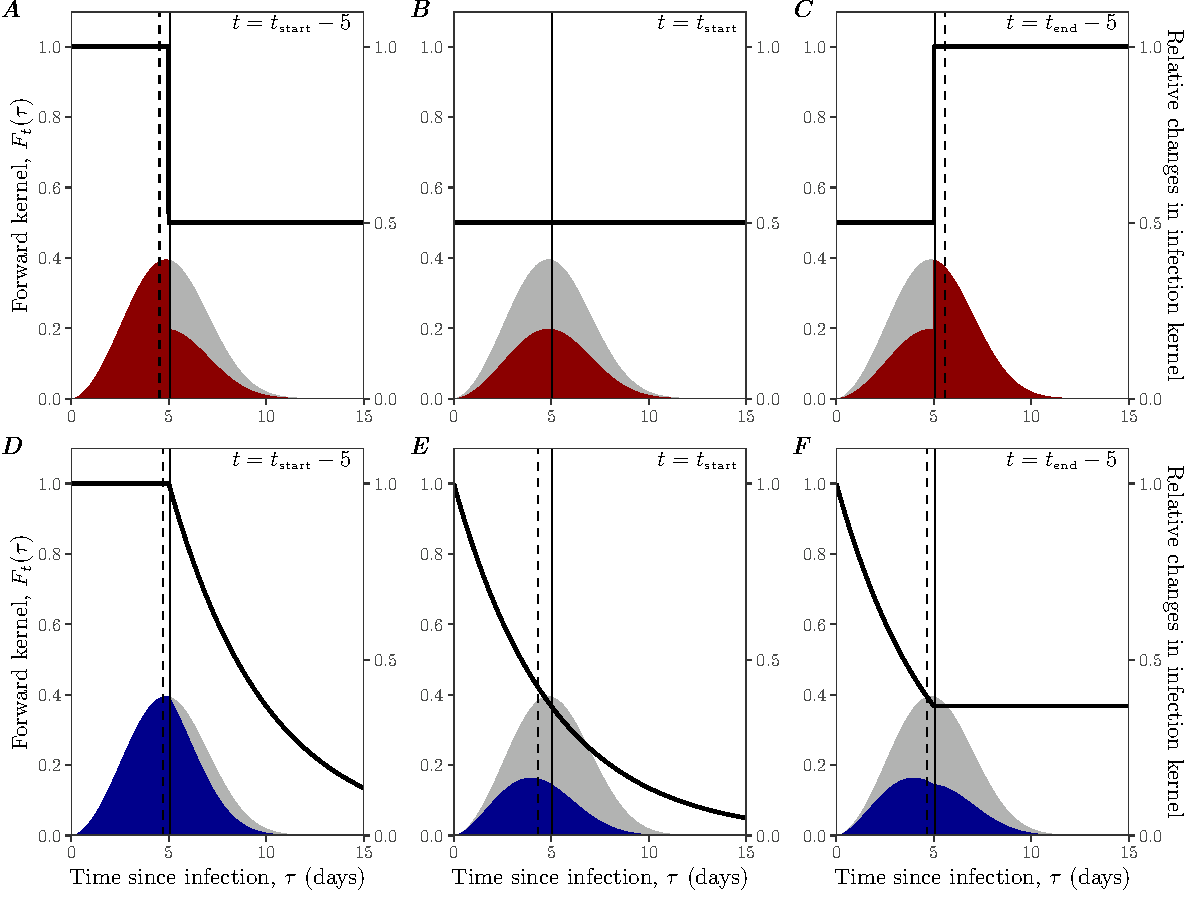
\includegraphics[width=1\textwidth]{pop_ind_compare.pdf}
\caption{
\textbf{I'm a caption}
}
\label{fig:indpop}
\end{figure}

To model the impact of intervention during an ongoing epidemic, we first distinguish population-based interventions, which equally affect the transmission potential of all infected individuals regardless of their time of infection, from individual-based interventions, which target each individual and therefore depend on the time of infection.
Population-based interventions can be thought of as interventions that reduce the transmission rate and include social distancing, school closures, and vaccination.
Individual-based interventions can be thought of as interventions that reduce the duration of infectious periods and include case identification and isolation.
Some interventions, like contact tracing, are conceptually analogous to individual-based interventions but are mathematically different from population- and individual-based interventions because they depend not only on the infection time of an infected individual but also on their infector's infection time;
for simplicity, we do not consider these at this stage.

Let $\PP(t)$ represent a population-level intervention that modulates the infection kernel multiplicatively at calendar time $t$ such that $\PP(t)=1$ corresponds to intervention that has no effect and $\PP(t) < 1$ corresponds to intervention that reduces transmission.
Then, the effective kernel under $\PP$ at calendar time $t$ can be written as:
\begin{equation}
K(t, \tau) = S(t) \PP(t) K(\tau).
\end{equation}
Likewise, the forward kernel of an individual infected at time $t$ under $\PP$ can be written as:
\begin{equation}
F_t(\tau) = S(t+\tau) \PP(t + \tau) K(\tau).
\end{equation}
Here, we see that population-level intervention has same impact on transmission dynamics as susceptible depletion.
This intervention is also strength-like because \swp{...}.
Since we assume that population-level internvention affects infection kernel multiplicatively, it is straightforward to model multiple interventions occuring throughout an epidemic: $\PP(t) = \prod_{i=1}^n \PP_i(t)$.

For example, a social distancing measure that reduces transmission potential by a factor of $1/\phi$ between time \tstart and \tend can be modeled as:
\begin{equation}
\PP(t) = \begin{cases}
1 & t < \tstart\\
\phi & \tstart \leq t < \tend\\
1 & \tend \leq t
\end{cases}.
\end{equation}
\fref{indpop}A--C illustrates the impact of such intervention on the forward kernel of an individual infected 5 days before $\tstart$, at $\tstart$, and 5 days before $\tend$ (assuming $S(t) \approx 1$).
Population-level interventions can take effect immediately and sharply reduce transmission (\fref{indpop}A);
likewise, lifting the intervention can, in theory, cause the forward kernel to return back to normal immediately (\fref{indpop}C).
Even though the exact shape of the kernel depends on the time of infection and when the intervention was introduced relative to the infection time, the relative impact of intervention in reducing transmission at any given time (by a factor of $1/\phi$) does not vary across individuals (\fref{indpop}A--C).
Such intervention also has direct effects on realized generation intervals:
implementing (lifting) intervention decreases (increases) future transmission potential and therefore decreases (increases) the mean realized generation interval (\fref{indpop}A,C).
If an individual is infected after \tstart (and much earlier than \tend), this intervention simply reduces the entire kernal by a constant amount and has no effect on realized generation intervals.
This mechanism explains and further generalizes how susceptible depletion leads to contraction of generation intervals in a homogeneously mixing population. 

On the other hand, individual-based intervention $\II(t, \tau)$, such as case isolation, targets each infected individual and therefore depends on calendar time $t$ as well as time since infection $\tau$.
In particular, we interpret $\II(t,\tau)$ as the probability that an individual infected $\tau$ time units ago has not been isolated by calendar time $t$ such that $\II(t, \tau) < 1$ represents reduction in transmission.
In this case, the effective kernel under $\II$ at calendar time $t$ is given by:
\begin{equation}
K(t, \tau) = S(t) \II(t, \tau) K(\tau).
\end{equation}
Likewise, the forward kernel of an individual infected at time $t$ under $\II$ can be written as:
\begin{equation}
F_t(\tau) = S(t+\tau) \II(t+\tau, \tau) K(\tau).
\end{equation}
This intervention is speed-like because its effectiveness depends on how fast we can isolate infected individuals.

For example, given hazard $h(\tau)$ of being isolated, the probability that an individual infected at time $t$ has not been isolated by $\tau$ time units after infection given that the individual-based intervention takes place between time \tstart and \tend depends on the amount of time the individual has been exposed to this intervention.
If the individual was infected before $\tstart$, they will not be isolated until after $\tstart$.
If the individual was infected after $\tend$, they will never be isolated.
Therefore, such probability can be modeled as:
\begin{equation}
\II(t+\tau, \tau) = \begin{cases}
1 & t < \tstart-\tau \\
\exp\left(- \int_{\max(0, \tstart - t)}^{\min(\tau, \tend-t)} h(s)\dd{s} \right) & \tstart-\tau \leq t < \tend \\
1 & \tend \leq t
\end{cases}
\end{equation}
Like population-level intervention, multiple individual-level interventions can be modeled using competing hazards ($h(\tau)=\sum_{i=1}^m h_i(\tau)$), which in turn can be expressed as product of interventions: $\II(t,\tau) = \prod_{i=1}^n \II_i(t,\tau)$.
\fref{indpop}D--E illustrates the impact of a single individual-based intervention with constant hazard on the forward kernel of an individual infected 5 days before $\tstart$, at $\tstart$, and 5 days before $\tend$ (assuming $S(t) \approx 1$).
Unlike the population-level intervention, individual-level internvetion does not take effect immediately;
that is, the rate at which an infected individual generates a secondary case at time $\tstart$ (e.g., $F_t(\tstart-t)$ in \fref{indpop}D; more generally, $K(\tstart, \tau)$) remains unaffected by the intervention because it takes time to identify and isolate infected individuals.
On the other hand, when the intervention is lifted at $\tend$, the value of the kernel at calendar time $\tend$ ($F_t(\tend-t)$ in \fref{indpop}F; more generally, $K(\tend, \tau)$) remains unchanged because some fraction of infected individuals have already been isolated.
In general, individual-based interventions shorten realized generation intervals because they prevent late transmission (\fref{indpop}D--E).

Finally, given (possibly multiple) population- and individual-based interventions, $P(t)$ and $I(t, \tau)$, the effective kernel can be written as:
\begin{equation}
K(t, \tau) = S(t) \PP(t) \II(t,\tau) K(\tau).
\end{equation}
The corresponding forward kernel can be written as:
\begin{equation}
F_t(\tau) = S(t+\tau) \PP(t + \tau) \II(t+\tau, \tau) K(\tau).
\end{equation}
Therefore, the dynamics of $S(t)$ and $i(t)$ can be now written as:
\begin{equation}
\begin{aligned}
\frac{\mathrm{d}S}{\mathrm{d}t} &= - i(t),\\
i(t) &= \int_0^\infty F_{t-\tau}(\tau) i(t-\tau) \dtau,\\
&=\int_0^\infty  K(t,\tau) i(t-\tau)\dtau,\\
&= S(t) \PP(t) \int_0^\infty \II(t, \tau) K(\tau) i(t-\tau)\dtau.
\end{aligned}
\end{equation}

\subsection{Quantifying changes in the reproduction number}

The impact of intervention is often measured by the instantaneous reproduction number $\RR(t)$, which is defined as the average number of secondary cases caused by a primary case infected at time $t$ given conditions at time $t$:
\begin{equation}
\RR(t) = \int_0^\infty K(t, \tau) \dtau.
\end{equation}
Since $\RR(t)$ measures conditions at time $t$, we expect to observe changes in $\RR(t)$ as soon as intervention is implemented.
While Cori et al have popularized the estimation of $\RR(t)$ via the R package EpiEstim, 


We argue that this has to be done by looking backward from the time of infection: by comparing the ratio of current incidence at time $t$ with previous incidence at time $t-\tau$ multiplied by their current infectiousness at time $t$.
This ratio is often referred to as the instantaneous reproduction number $\RR(t)$.

In order to define the instantaneous reproduction number $\RR(t)$, we want to account for changes in the underlying generation-interval distribution due to intervention.
Thus, we define effective generation-interval distribution $\geff(t, \tau)$ which accounts for the individual-level intervention.
Given time of infection $t'$ and time since infection $\tau$, we have:
\begin{equation}
\geff(t', \tau)= \frac{\beta(\tau)I(t'+\tau,t')}{\int_0^\infty \beta(x)I(t'+x,t') \dx}.
\end{equation}
Then, we can rewrite Eq~?? as:
\begin{equation}
\begin{aligned}
\frac{\mathrm{d}S}{\mathrm{d}t} &= - i(t),\\
i(t) &=  \mathcal R(t) \int_0^\infty i(t-\tau)  \geff(t-\tau, \tau) \dtau.
\end{aligned}
\end{equation}
Here, the instantaneous reproduction number $\RR(t)$ is defined as:
\begin{align}
\RR(t) &= S(t) P(t) \int_0^\infty I(t,t-\tau) \beta(\tau) d\tau,\\
&= \Ro S(t) P(t) \int_0^\infty I(t,t-\tau) g(\tau) d\tau,
\end{align}
which depends on the proportion of the susceptible population and proportional reduction in the intrinsic infectivity of an individual, weighted by the intrinsic generation-interval distribution.
Then, we can estimate the instantaneous reproduction number as follows:
\begin{equation}
\RR(t)= \frac{i(t)}{\int_0^\infty i(t-\tau) \geff(t-\tau, \tau) \dtau}.
\end{equation}
This definition of the instantaneous reproduction number contrasts with the widely used definition that assumes that the underlying generation-interval distribution remains constant.

Given incidence between time $0$ and $t-\epsilon$ for $\epsilon > 0$, we can also calculate the proportional reduction $p(t)$ in true incidence $i(t)$ at time $t$ compared to incidence that we would get in the absence of intervention:
\begin{equation}
p(t) = \frac{S(t) P(t) \int_0^\infty i(t-\tau) I(t,t-\tau) \beta(\tau) \dtau}{S(t) \int_0^\infty i(t-\tau) \beta(\tau) \dtau}.
\end{equation}
By substituting true incidence $i(t)$ in the numerator and rearranging, we get a familiar expression for the estimator for $\RR(t)$, which we refer to as $\tsub{\RR}{prop}(t)$ that depends on the proportion of the susceptible population and proportional reduction in incidence:
\begin{equation}
\tsub{\RR}{prop}(t) = \Ro S(t) p(t) = \frac{i(t)}{\int_0^\infty i(t-\tau) g(\tau) \dtau}.
\end{equation}




\end{document}
